\documentclass{allertonproc}
\usepackage{amsmath}
\usepackage{graphicx}
\usepackage{epsfig}
\usepackage{cite}
\usepackage{placeins}
\usepackage{fancyhdr}
\renewcommand{\topfraction}{0.9}	% max fraction of floats at top
    \renewcommand{\bottomfraction}{0.9}	% max fraction of floats at bottom
    %   Parameters for figures in places on TEXT pages (not float pages):
    \setcounter{topnumber}{2}
    \setcounter{bottomnumber}{2}
    \setcounter{totalnumber}{4}    
\begin{document}
\bibliographystyle{IEEEtran}
\title{ TRANSMISSION LINE MODEL FOR MICROSTRIP LINE ABOVE A
PERIODIC HIGH-IMPEDANCE SURFACE GROUND PLANE}
\author{K.~C.~Kerby-Patel\\The MITRE Corporation, Bedford, MA\\kkerby@mitre.org}
\maketitle
\begin{abstract}
High impedance surfaces, including electromagnetic bandgap surfaces, have proven useful in the design of low-profile antennas. However, the surface and antenna are typically designed separately and then combined, which results in detuning of the antenna because the method does not account for near-field interaction between the antenna and the high-impedance surface. This paper describes a transmission line model which captures the guided wave behavior of the combined antenna-ground structure by representing it as a microstrip line above a high-impedance ground plane.

The model consists of a periodic transmission line structure. A transmission line, which represents the microstrip line, is coupled to a periodic structure of transmission line resonators representing the high-impedance surface features. The model predicts the impedance and dispersion behavior of the combined structure. A detailed description of the transmission line model is provided, followed by comparison of its predictions against simulated results.
\end{abstract}
\section{Introduction}
High impedance surfaces, including electromagnetic bandgap surfaces, have
proven useful in the design of low-profile antennas. However, the surface and antenna
are typically designed separately and then combined, which results in detuning of the
antenna because the method does not account for near-field interaction between the
antenna and the high-impedance surface. We would like to have a model that incorporates that effect and is simple enough to be used in the first iteration of the design process.

Transmission line models lend themselves to this goal; while more precise prediction is possible using simulation, a transmission line based model lends itself to physical insight about the structure and preliminary prediction of behavior.   Our goal is to develop a model, like the simple transmission line model for the microstrip patch antenna \cite{munson}, that can be used as a tool for prediction and design.

\section{Model Description}
\subsection{The Unit Cell}
A microstrip line backed by a high-impedance surface, which we will call HIstrip for brevity, is a periodic structure.  To characterize the propagation constant and impedance of a long section of such a line, we follow a Bloch analysis technique as described in Pozar \cite{pozar}. The structure is represented as set of stacked transmission lines, where one of the conductors is loaded periodically by reactances that represent the grounding vias and the gaps between adjacent patches. 

Multiconductor transmission lines have been thoroughly discussed by Faria \cite{fariabook} and Paul \cite{paulbook}, and were recently used by Elek and Eleftheriades to analyze wave propagation on a shielded EBG surface \cite{elek}.  The top conductor is Terminal 1, the patch layer is Terminal 2, and the ground plane is the ground terminal (Terminal 0) for the multiconductor line structure.  We define voltage $V_1$ between Terminal 1 and ground, voltage $V_2$ between Terminal 2 and ground, and current going into the ports. The current at Port 2 is reversed for ABCD matrices, as is typical.

\begin{figure}[tbp]
\begin{center}
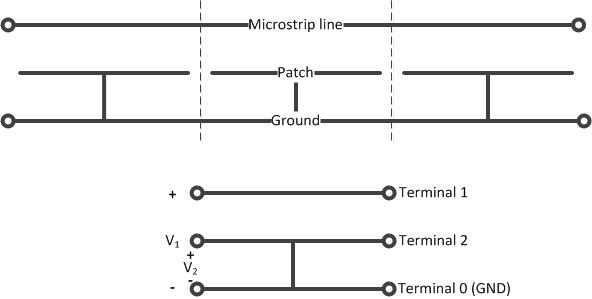
\includegraphics[width=4in]{physstructure}
\caption{Cross-sectional view of the physical HIstrip structure.  Dashed lines represent the port reference planes of the unit cell.  At each port, Terminal 1 is defined on the top microstrip line and Terminal 2 is defined on the row of patches.}
\label{physicalstructure}
\end{center}
\end{figure}
\begin{figure}[thb]
\begin{center}
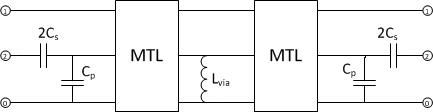
\includegraphics[width=4in]{MTL_circuitmodel}
\caption{Circuit model for the unit cell of a microstrip line backed by a Sievenpiper high-impedance surface, including multiconductor transmission line (MTL) segments.  }
\label{tlmodel}
\end{center}
\end{figure}
A diagram of the physical structure is shown in Figure \ref{physicalstructure},  and the resulting transmission line model is shown in Figure \ref{tlmodel}. We will represent the gap as a $\pi$-network of capacitors using Hammerstad's empirically derived formula for the reactance due to a gap in microstrip \cite{hammerstad}.  The inductance due to the grounding via is determined by Goldfarb and Pucel's formula \cite{goldfarb}.  We can choose the reference plane of the unit cell arbitrarily, so we place it in the center of the gap between two of the high impedance surface's patches.  This is similar to how such a structure is usually excited in practice, and it helpfully creates a symmetric unit cell.  We have not yet estimated the multiconductor transmission line's parameters, which will be discussed next.

\subsection{Estimating Parameters for the Multiconductor Line}
\begin{figure}[tb]
\begin{center}
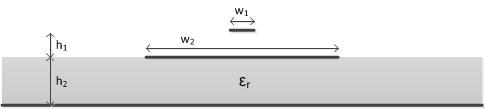
\includegraphics[width=4in]{ustrip_example}
\caption{Diagram of stacked microstrip line structure for example multiconductor line parameter derivation. The width of the microstrip line is $w_1$, patch width is $w_2$ and the dielectric constant of the substrate is $\epsilon_r$.  In our example, the patches are printed on the substrate and the microstrip line is suspended in air.}
\label{ustrip_example}
\end{center}
\end{figure}
We can use well-known formulas for the per-unit-length capacitance and inductance of microstrip line to estimate the parameters of the multiconductor transmission line \cite{microstrip}. We assume the conductors are arranged as shown in Figure \ref{ustrip_example}. If the patch width is much wider than the upper microstrip width (or if there are multiple rows of patches), it is reasonable to assume that $C_{11}$ is negligible compared to $C_{12}$.  Then the mutual capacitance matrix can be approximated using only $C_{12}$ and $C_{22}$, which can be derived from design equations for microstrip line \cite{microstrip}.
\begin{equation}
\mathbf{C} = \begin{bmatrix}C_{11}+C_{12} & -C_{12} \\ -C_{12} & C_{22}+C_{12} \end{bmatrix} \approx \begin{bmatrix}C_{12} & -C_{12} \\ -C_{12} & C_{22}+C_{12} \end{bmatrix}
\end{equation}

Next, we make use of the property (from \cite{fariabook}) that the mutual inductance matrix can be derived from the mutual capacitance matrix of the same structure with all dielectrics removed, $\mathbf{C_0}$.  We can derive $\mathbf{C_0}$ from microstrip design equations as well, and it will have the same structure as $\mathbf{C}$.
\begin{equation}
\mathbf{L} = \mu_0 \epsilon_0 \mathbf{C_0}^{-1}
\end{equation}

We derive the terminal characteristic impedance matrix following the method from \cite{fariabook},
\begin{equation}
\mathbf{\Gamma} = \textsc{sqrtm}\left(-\omega^2\mathbf{L}\mathbf{C}\right)
\end{equation}
\begin{equation}
\mathbf{Z_0} = \mathbf{\Gamma}^{-1}j\omega\mathbf{L}
\end{equation}
where $\textsc{sqrtm}$ denotes the matrix square root.  A consequence of our omission of $C_{11}$ is that $Z_{21} = Z_{12} = Z_{22}$, which is approximate but not precisely true in practice, as we will see from an example.  We will also tend to slightly overestimate $Z_{11}$.  For wider upper lines or narrower patch widths, it may be more appropriate not to omit $C_{11}$.  However, since the physical problem of interest includes a 2D periodic lattice of patches, the impedance matrix we obtain through simulation of a simple stacked microstrip structure may actually overestimate $C_{11}$ for a HIstrip structure by using only the width of a single patch for the middle layer conductor.

Consider again the uniform stacked microstrip line structure from Figure \ref{ustrip_example}.  In our example case, $w_1 = 0.01$ m, $w_2 = 0.12$ m, $h_1 = 0.02$ m, $h_2 = 0.04$ m, and $\epsilon_r = 2.2$. Using the ``Port $Z_0$'' capability in Ansoft HFSS \cite{HFSS}, we can simulate the characteristic impedance matrix of this structure for comparison with our predicted values.  The results are shown in Figures \ref{Zchar11}-\ref{Zchar22}.  Since the characteristic impedance matrix is symmetric, $Z_{21}$ is not plotted because it is equal to $Z_{12}$.  The imaginary parts of the characteristic impedances calculated by HFSS are approximately zero, and those calculated by our method are exactly zero.  As one might expect due to our omission of $C_{11}$, the model overestimates $Z_{11}$ and does not capture a slight difference between $Z_{12}$ and $Z_{22}$.
\begin{figure}[bp]
\begin{center}
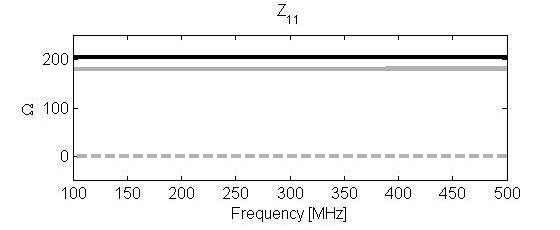
\includegraphics[width=4in]{Zchar11}
\caption{Real (solid lines) and imaginary (dashed lines) part of $Z_{11}$ from the characteristic impedance matrix for the multiconductor line structure shown in Figure \ref{ustrip_example}, as calculated using the microstrip design equations (black) and by Ansoft HFSS simulation (gray).}
\label{Zchar11}
\end{center}
\end{figure}
\begin{figure}[bpt]
\begin{center}
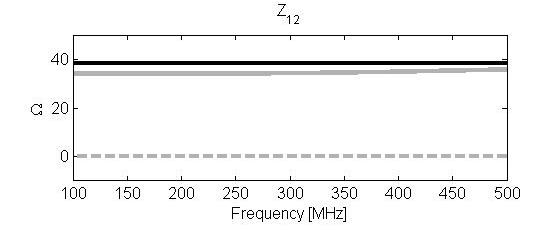
\includegraphics[width=4in]{Zchar12}
\caption{Real (solid lines) and imaginary (dashed lines) part of $Z_{12}$ from the characteristic impedance matrix for the multiconductor line structure shown in Figure \ref{ustrip_example}, as calculated using the microstrip design equations (black) and by Ansoft HFSS simulation (gray).}
\label{Zchar12}
\end{center}
\end{figure}
\begin{figure}[tpb]
\begin{center}
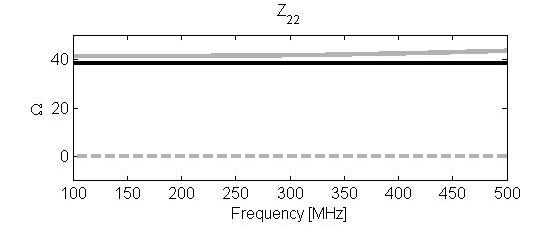
\includegraphics[width=4in]{Zchar22}
\caption{Real (solid lines) and imaginary (dashed lines) part of $Z_{22}$ from the characteristic impedance matrix for the multiconductor line structure shown in Figure \ref{ustrip_example}, as calculated using the microstrip design equations (black) and by Ansoft HFSS simulation (gray).}
\label{Zchar22}
\end{center}
\end{figure}

\subsection{ABCD Matrix Analysis of the Unit Cell}
In the previous section, we developed a multiconductor transmission line model for the HIstrip line shown in Figure \ref{physicalstructure}.  Now we analyze the periodic structure, following the method outlined in \cite{faria2004}.  We begin by writing the multiconductor $ABCD$ matrix for each component.

% write out all the ABCD matrices
\begin{equation}
\mathbf{L_{via}} = \begin{bmatrix}1 & 0 & 0 & 0\\0 & 1 & 0 & 0\\ 0 & 0 & 1 & 0\\ 0 & 1/j\omega L_{via} & 0 &1\end{bmatrix}
\end{equation}
\begin{equation}
\mathbf{C_s} = \begin{bmatrix}1 & 0 & 0 & 0\\0 & 1 & 0 & 1/j\omega C_s\\ 0 & 0 & 1 & 0\\ 0 & 0 & 0 &1\end{bmatrix}
\end{equation}
\begin{equation}
\mathbf{C_{p2}} = \begin{bmatrix}1 & 0 & 0 & 0\\0 & 1 & 0 & 0\\ 0 & 0 & 1 & 0\\ 0 & j\omega C_{p2} & 0 &1\end{bmatrix}
\end{equation}

One could also include an upper shunt capacitance at the gap, transforming the $\pi$ network into an H shape.  The value of the capacitance can be estimated using the upper microstrip line's dimensions in Hammerstad's expression for the gap reactance.  This approach is imperfect because it assumes a gap in the line, rather than in the ``ground,'' but in our tests the model turns out not to be very sensitive to the value, or even existence, of this capacitor.
\begin{equation}
\mathbf{C_{p12}} = \begin{bmatrix}1 & 0 & 0 & 0\\0 & 1 & 0 & 0\\ j\omega C_{p12} & -j\omega C_{p12} & 1 & 0\\ -j\omega C_{p12} & j\omega C_{p12} & 0 &1\end{bmatrix}
\end{equation}

The multiconductor transmission line section is represented by 
\begin{equation}\label{MTLsection}
\mathbf{M_{MTL}} = \begin{bmatrix}\mathbf{T}\cosh( \mathbf{g} w_2/2 )\mathbf{T}^{-1}   & \mathbf{T}\sinh( \mathbf{g} w_2/2 )\mathbf{T}^{-1}\mathbf{Z_0}\\ \mathbf{Y_0}\mathbf{T}\sinh( \mathbf{g} w_2/2 )\mathbf{T}^{-1} & \mathbf{T}\cosh( \mathbf{g} w_2/2 )\mathbf{T}^{-1} \end{bmatrix}
\end{equation}
% describe how to get the prop constants and modal impedances, and what the transformation matrices mean
where $\mathbf{g}$ is the diagonal matrix of modal propagation constants, and $\mathbf{T}$ is the transformation matrix that transforms the modal voltages $\hat{\mathbf{v}}$ into the terminal voltages $\mathbf{v}$.  \mbox{Equations \ref{gammaLC}-\ref{vT}} describe the relationships between these quantities that are necessary to determine the multiconductor transmission line's ABCD matrix.
\begin{equation}\label{gammaLC}
\mathbf{T}\mathbf{g}^2\mathbf{T}^{-1} = -\omega^2\mathbf{L}\mathbf{C} = \mathbf{\Gamma}^2
\end{equation}
\begin{equation}
\mathbf{\Gamma} = \mathbf{T}\mathbf{g}\mathbf{T}^{-1}
\end{equation}
\begin{equation}\label{vT}
\mathbf{v} = \mathbf{T}\hat{\mathbf{v}}
\end{equation}

More details on these and other relationships between the multiconductor transmission line parameters can be found in \cite{fariabook} or \cite{paulbook}.  When finding the values of the modal propagation constants from the per-unit-length inductance and capacitance matrices $\mathbf{L}$ and $\mathbf{C}$, it is important to ensure proper choice of roots by finding the eigenvalues of $-\omega^2\mathbf{LC}$, then choosing the square root of those eigenvalues to obtain $\mathbf{g}$.  The eigenvalues of $\mathbf{\Gamma}$ are $\mathbf{g}$, but finding $\mathbf{g}$ this way introduces a sign ambiguity.

Finally, the $ABCD$ matrix of the unit cell structure is 
\begin{equation}
\mathbf{M_{cell}} = \mathbf{C_s}\ \mathbf{C_{p2}} \ \mathbf{M_{MTL}} \ \mathbf{L_{via}} \ \mathbf{M_{MTL}} \ \mathbf{C_{p2}} \ \mathbf{C_s} = \begin{bmatrix} \mathbf{A} & \mathbf{B} \\ \mathbf{C} & \mathbf{D} \end{bmatrix}
\end{equation}

The method used to derive $\mathbf{T}$, $\mathbf{g}$, and $\mathbf{Z_0}$ for the uniform multiconductor line has been generalized to nonuniform lines in \cite{faria2004}.  The key difference is that we then obtain different voltage transformation matrices $\mathbf{T_0}$ and $\mathbf{T_\ell}$ (and their corresponding current transformation matrices $\mathbf{W_0}$ and $\mathbf{W_\ell}$)  for either end of the unit cell that are not necessarily equal.  $\mathbf{T_0}$ is the eigenvector matrix of $\mathbf{B}\mathbf{C}^T$, and $\mathbf{T_\ell}$ is the eigenvector matrix of $\mathbf{B}^T\mathbf{C}$.

\section{Example}
Now we are prepared to compare the circuit model's predictions against a full-wave simulation.  The high-impedance surface has substrate $\epsilon_r = 2.2$, patch width $w_2 = 0.12$ m, gap width 0.02 m, substrate height 0.04 m, and via radius 1.5875 mm.  The sum of the patch and gap widths equals the unit cell length $a = 0.14$ m.  The microstrip line is 0.01 m wide and suspended in air 0.02 m above the patches.    The structure is nominally designed at 300 MHz, so distances in meters are equivalent to distances in wavelengths.  The HFSS model that was used to simulate the HIstrip structure is shown in Figure \ref{HFSSmodelpic}. 
\begin{figure}[htb]
\begin{center}
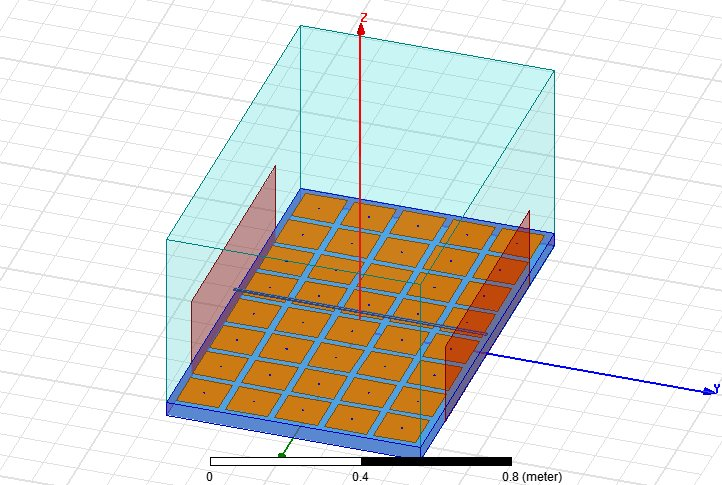
\includegraphics[width=4in]{HFSSmodelpic}
\caption{HFSS model of microstrip line above a Sievenpiper high-impedance surface.}
\label{HFSSmodelpic}
\end{center}
\end{figure}

 In order to unambiguously derive the propagation constant and Bloch impedance on this periodic structure, two structures with mutually prime numbers of unit cells were simulated (4 cells and 5 cells) following the technique described in \cite{valerio}.  It should be pointed out that these simulated structures had only two terminals (the microstrip line and ground) at the ports, rather than the three terminals in our multiconductor line model.  The patch layer effectively had an open-circuit termination at the plane of the wave port due to the Bloch condition applied in post-processing.  The result is that we only have access to $Z_{11}$.

We use the microstrip-based approximations to estimate all lumped components and transmission line parameters.  We obtain $L_{via} = 19.8$ nH.  Hammerstad's expression for gap capacitance contains a slight frequency dependence, so $C_s$ increases from 1.23 pF at 100 MHz to 1.65 pF at 500 MHz.  Similarly, $C_{p2}$ increases from 2.33 pF to 2.44 pF over the band.  Lastly, the per-unit-length parameters of the multiconductor line are derived from the microstrip design equations of \cite{microstrip}.
\begin{equation}
\mathbf{L} = \begin{bmatrix}791 &  234\\  234&  234\end{bmatrix} \mathrm{nH/m}
\end{equation}
\begin{equation}
\mathbf{C} =  \begin{bmatrix}20.0 & -20.0\\-20.0 & 110\end{bmatrix} \mathrm{pF/m}
\end{equation}

% present results from a simulated example
The Bloch modal propagation constant for the HFSS model is shown in Figure \ref{HFSS_dispersion}.  Only one propagation constant is shown because the HFSS model's waveports did not include a terminal on Terminal 2.  Bloch analysis predicts two modal propagation constants, $\gamma_1$ and $\gamma_2$.  Each $\gamma_i$ consists of an attenuation constant $\alpha_i$ and a phase constant $\beta_i$.  
\begin{equation}
\gamma_i = \alpha_i+j\beta_i
\end{equation}

Figure \ref{ckt_dispersion} shows the Bloch modal propagation constants predicted by the circuit model.  This dispersion diagram is shown one-sided to emphasize the fact that the two modal phase constants, $\beta_1$ and $\beta_2$ are equal and opposite in the stopband. The circuit model underestimates the frequency of the stopband by about 8\%, with maximum $|\beta|$ occurring at 221 MHz as compared to 239 MHz in the HFSS simulation.  However, the circuit model captures the major features of the dispersion diagram, including a narrow leaky-wave band above the stopband that was also observed in \cite{besthanna}.
\begin{figure}[htbp]
\begin{center}
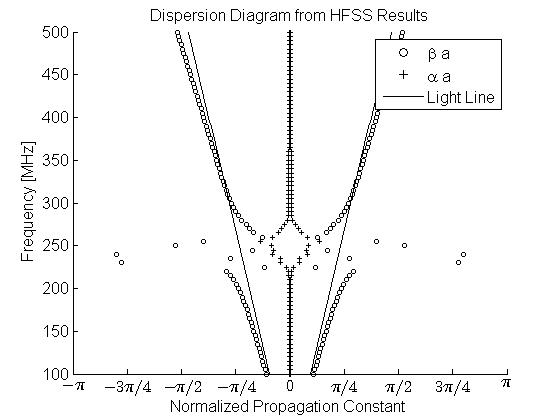
\includegraphics[width=4in]{HFSS_dispersion}
\caption{Bloch mode propagation constants from HFSS simulation.}
\label{HFSS_dispersion}
\end{center}
\end{figure}
\begin{figure}[htbp]
\begin{center}
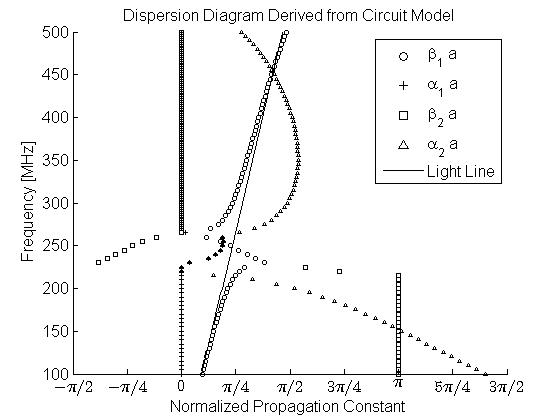
\includegraphics[width=4in]{ckt_dispersion}
\caption{Bloch mode propagation constants calculated from circuit model.}
\label{ckt_dispersion}
\end{center}
\end{figure}
\FloatBarrier

\begin{figure}[hbtp]
\begin{center}
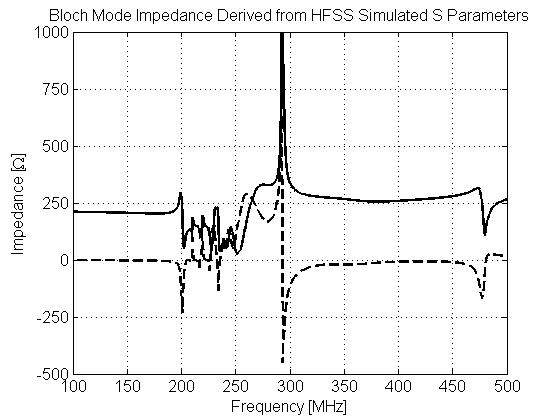
\includegraphics[width=4in]{HFSSZbloch}
\caption{Bloch impedance at Terminal 1 from HFSS simulation.}
\label{HFSSZbloch}
\end{center}
\end{figure}
\begin{figure}[htbp]
\begin{center}
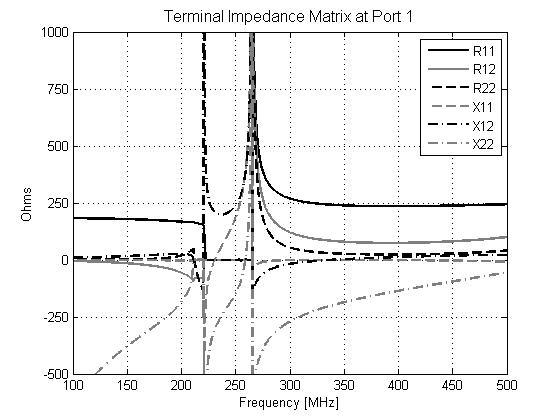
\includegraphics[width=4in]{cktZbloch}
\caption{Bloch mode impedance matrix components calculated from circuit model.}
\label{cktZbloch}
\end{center}
\end{figure}
The Bloch modal impedance for the HFSS model is shown in Figure \ref{HFSSZbloch}.  The wave ports did not have a terminal on Terminal 2, so only the Bloch impedance for Terminal 1 is included.  Figure \ref{cktZbloch} shows the Bloch impedance matrix as predicted by the circuit model.  The circuit model captures major features of the impedance antiresonance and predicts the line impedance correctly away from the antiresonance, but underestimates the frequency of the antiresonance by approximately 10\% (predicted 265 MHz, as compared to 292 MHz in simulation).  It is interesting to note that the impedance antiresonance does not occur within the stopband of the dispersion diagram, but slightly above it, in both the HFSS simulation and the circuit model's prediction.  

The circuit model and HFSS simulation both indicate that the Bloch impedance of the HIstrip line away from the stopband is fairly stable over a wide bandwidth.  Its value is  approximately the same as the characteristic impedance of the upper line alone. Away from the stopband, the propagation constant on the HIstrip line is also not significantly different from the standard microstrip line.  Most HIstrip-based antennas operate in this region, where we have just determined that the HIstrip line structure behaves essentially the same as standard microstrip line.  This leads us to ask what exactly is accomplished by the presence of the high impedance surface, since a standard wire antenna closely spaced to a ground plane is poorly matched while its HIstrip-based counterpart is not.  In order to address this question, the next section examines the effect of a high impedance ground plane on a simple dipole antenna.
\FloatBarrier

\section{Discussion}
We have pointed out that the Bloch impedance away from the stopband is approximately equal to the characteristic impedance of the upper line alone.  In that case, what is accomplished by the presence of the high impedance surface?  Recall that the Bloch impedance is based on an infinite series of unit cells, and realistic antenna designs never actually use an infinite structure.  The transmission-line resonator model of a microstrip antenna has a termination, $Z_{rad}$, which represents the radiation resistance of the antenna and the antenna's reactance.  In this section, we will make the argument that the contribution of the high-impedance surface is in how it modifies the apparent termination of the antenna structure. 

\begin{figure}[htbp]
\begin{center}
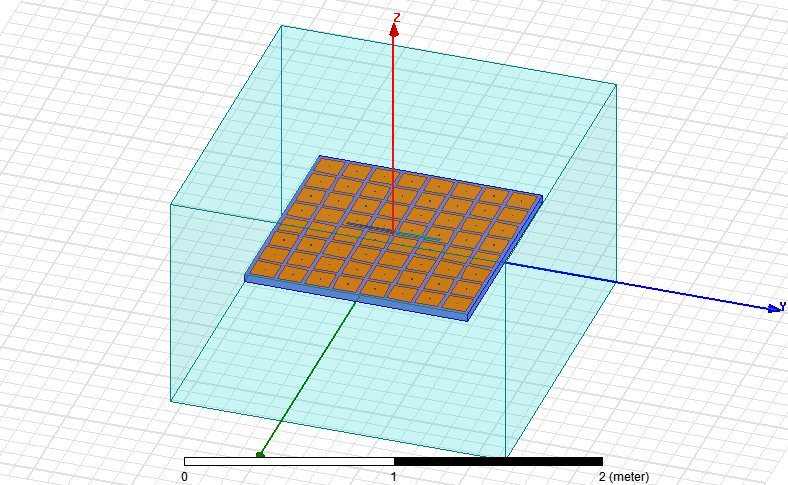
\includegraphics[width=4in]{HIstripDipoleModelPic}
\caption{HFSS model for high impedance surface backed dipole.}
\label{HIstripDipoleModelPic}
\end{center}
\end{figure}
\begin{figure}[htbp]
\begin{center}
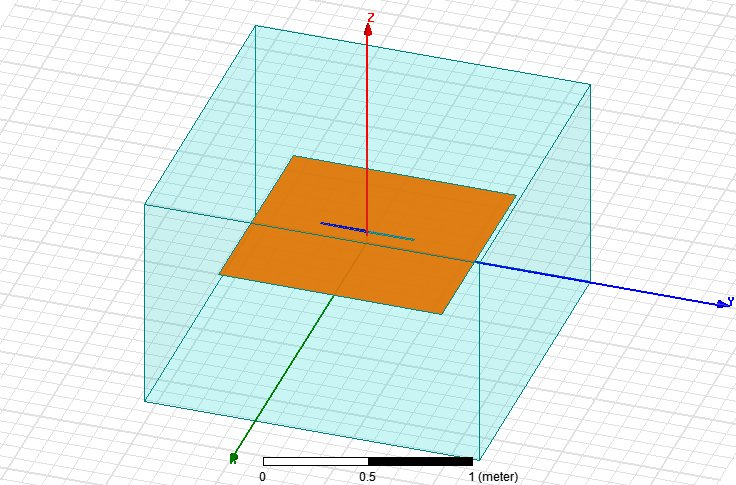
\includegraphics[width=4in]{NormalDipoleModelPic}
\caption{HFSS model for PEC-backed dipole.}
\label{NormalDipoleModelPic}
\end{center}
\end{figure}

We investigate the question with a pair of simulated tests.  The first model consists of a dipole antenna of length 0.47 m, constructed from the same HIstrip structure used in our modal analysis example.  The antenna is $h_1 = 0.02$ m above the high impedance surface.  The second test is another dipole antenna of the same dimensions, positioned the same distance $h_1 = 0.02$ m above a perfectly electrically conductive (PEC) ground plane.  The models are shown in Figures \ref{HIstripDipoleModelPic} and \ref{NormalDipoleModelPic}.  The HIstrip dipole is well matched at resonance, while the PEC-backed dipole is not matched (Figure \ref{dipoleS11graph}), despite having approximately the same transmission line parameters.

\begin{figure}[htbp]
\begin{center}
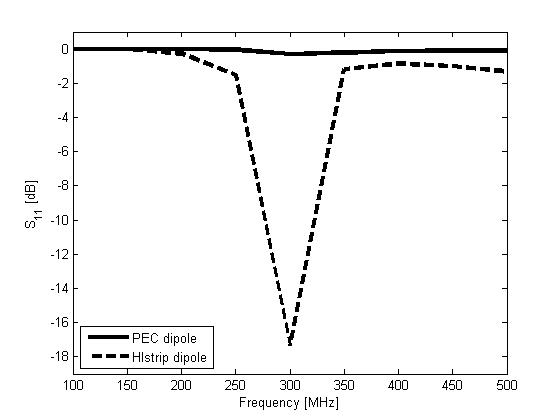
\includegraphics[width=4in]{dipoleS11graph}
\caption{$S_{11}$ from HFSS models for PEC-backed dipole (solid line) and HIstrip dipole (dashed line).}
\label{dipoleS11graph}
\end{center}
\end{figure}

If the line parameters are approximately the same, the difference must be in the termination of the line.  Assuming a simple model in which the antenna is a center-fed transmission line resonator and each end of the resonator is terminated by the radiation impedance, we can use the input impedance of the antenna model to estimate what that radiation impedance must be.  We include a length correction \cite{kirschning} to correct for the effect of fringing fields at the open ends of the line.  The resulting estimation is qualitatively useful but may be inaccurate near resonance, where the tangent term in the equation below is very sensitive to our choce of the length correction. Equation \ref{Zineqn} uses the input impedance looking into one side of the resonator, so that the total antenna input impedance is $Z_{in}/2$.
\begin{equation}\label{Zineqn}
Z_{rad} = Z_0\frac{Z_0-jZ_{in}\tan\beta(\ell+\Delta\ell)}{Z_{in}-jZ_0\tan\beta(\ell+\Delta\ell)}
\end{equation}

\begin{figure}
\begin{center}
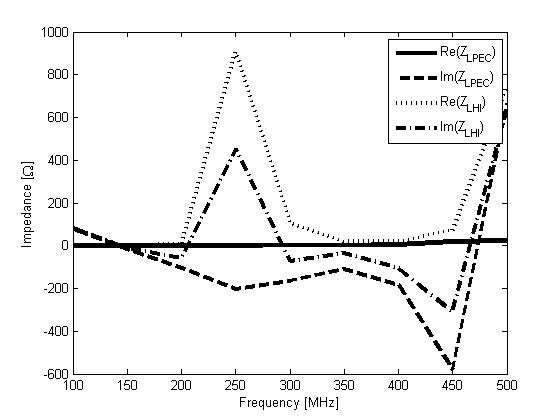
\includegraphics[width=4in]{Ztermgraph}
\caption{Radiation impedance calculated from input impedance of HFSS simulated antennas, backed by PEC ($R$ = solid line, $X$ =  dashed line) and high impedance surface ( $R$ = dotted line, $X$ = dot-dashed line).}
\label{Ztermgraph}
\end{center}
\end{figure}

The resulting estimated radiation impedances are shown in Figure \ref{Ztermgraph}.  The PEC-backed antenna has very low radiation resistance over the entire band, as we expect for a dipole near a PEC surface.  The high impedance backed antenna's radiation impedance tracks that of the PEC-backed antenna below the stopband, has a spike in the stopband, and has higher radiation resistance than the PEC-backed dipole above the stopband.  We may gain some insight as to the cause of this difference in radiation impedance by examining the surface currents on the ground plane in each case (Figures \ref{HIstripJsurf} and \ref{PECJsurf}).  The surface current in the high impedance ground plane case is distributed over a wider area at the resonant frequency, increasing the effective size of the antenna.

\begin{figure}
\begin{center}
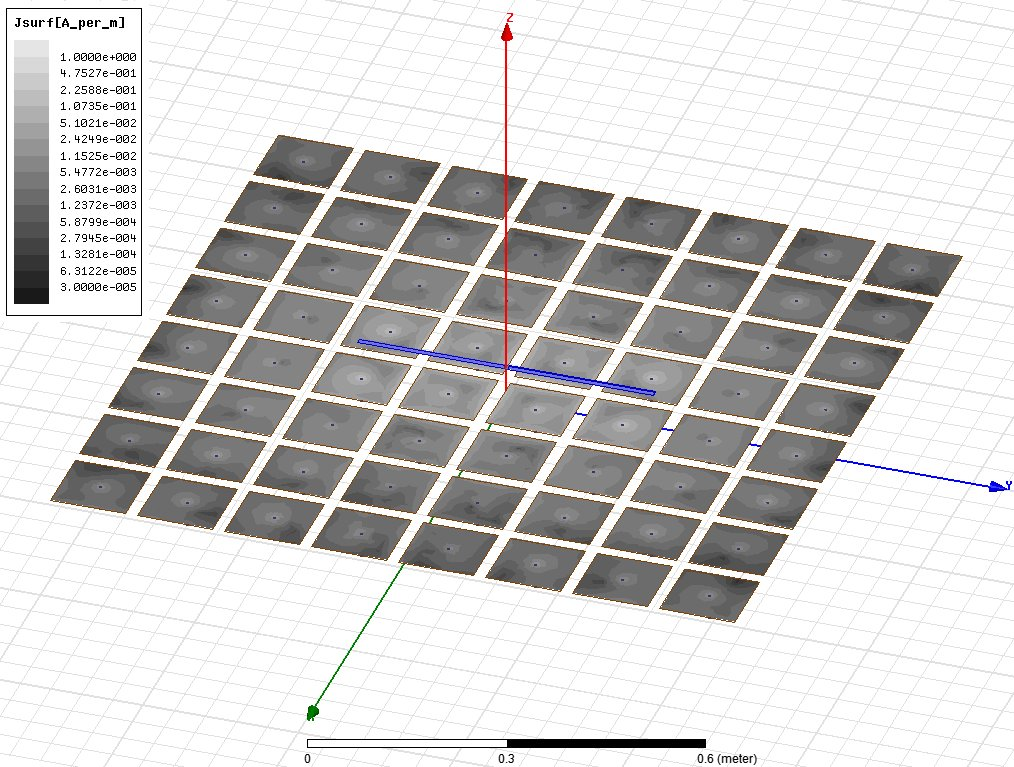
\includegraphics[width=4in]{HIstripJsurf}
\caption{Ground plane surface current log magnitude from HFSS model for high impedance surface backed dipole at resonance (300 MHz).}
\label{HIstripJsurf}
\end{center}
\end{figure}

\begin{figure}
\begin{center}
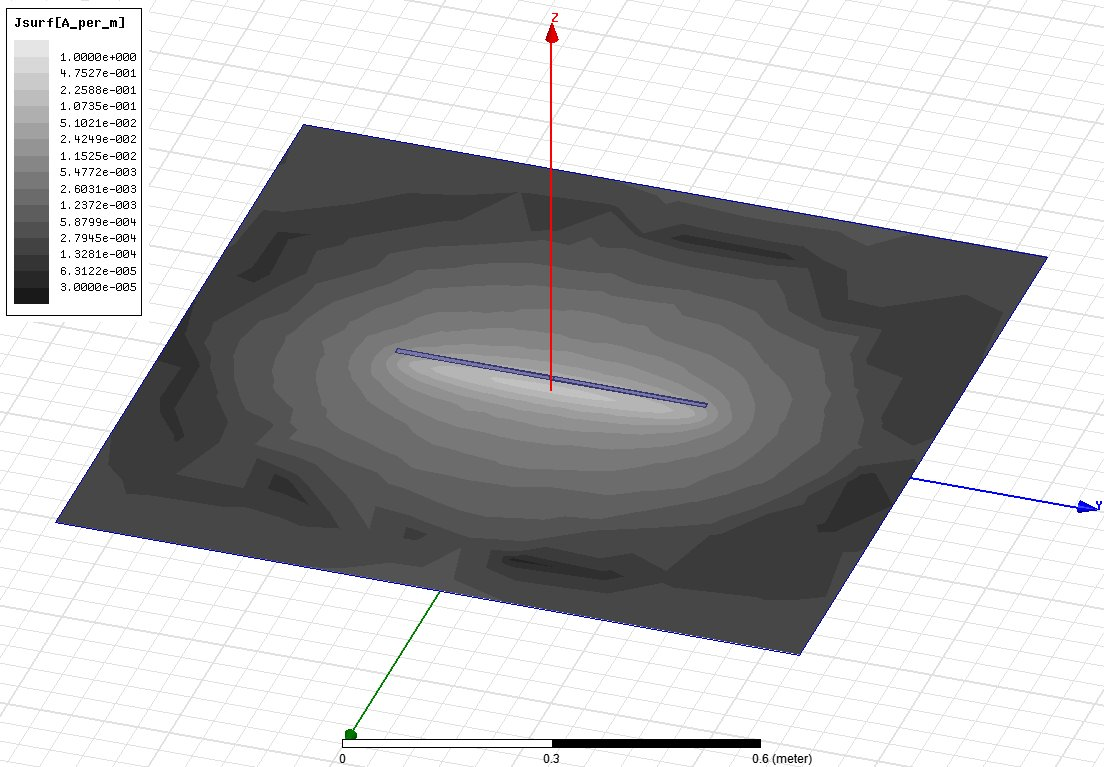
\includegraphics[width=4in]{PECJsurf}
\caption{Ground plane surface current log magnitude from HFSS model for PEC-backed dipole at resonance (300 MHz).}
\label{PECJsurf}
\end{center}
\end{figure}
\FloatBarrier
\section{Conclusion}
We have presented a circuit model that describes wave propagation on microstrip line above a high impedance surface. The circuit model predicts most features of the simulated results, including line impedance and modal propagation constants.  These results can be used predictively for low-profile antenna design. The circuit model does not capture certain finer details within the stopband, and tends to underestimate the stopband frequency slightly.  

The circuit model and full-wave simulation both demonstrated that, away from the stopband region, the Bloch impedance and propagation constant for the high impedance backed microstrip structure are nearly equal to the characteristic parameters of a standard microstrip line (as if the surface patches were replaced by a PEC ground plane).  Since most high impedance backed antennas operate away from the stopband region, this result implied that the main effect of the high impedance surface is not to modify propagation on the microstrip line, but to modify the effective termination of the antenna by changing the radiation impedance.   A preliminary investigation shows evidence to support this hypothesis, but further analysis is required to fully understand the effect.
\section{Acknowledgements}
Approved for Public Release; Distribution Unlimited. 13-2943\\ \copyright 2013-The MITRE Corporation. All rights reserved.

\bibliography{allertonrefs}{}
\end{document}